\chapter{Grundlagen}
\todo{Christian}
\section{A* Algorithmus}
Der A*-Algorithmus ist ein Wegfindungs-Algorithmus, der von Peter Hart, Nils Nilsson und Bertram Raphael entwickelt wurde. Sein Ziel ist es den schnellsten Weg in einem Grafen vom Startknoten zum Zielknoten zu finden. 
\subsection{Funktionsweise}
\begin{wrapfigure}{r}{2.5cm}
    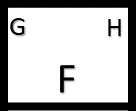
\includegraphics[width=1.5cm]{assets/aStarNode.png}
    \caption{Beispiel Node}
    \label{fig:aStarNode}
\end{wrapfigure}
Der Ausgangspunkt bildet ein zwei-dimensionales Array in dem es Felder gibt, die entweder Pfad und Hindernis darstellen. Es wird ein Start- sowie Zielfeld festgelegt. Beide sind dem Algorithmus während der Ausführung bekannt.Sobald das Spielfeld erstellt sowie ein Start- und Zielfeld gewählt wurde, sind die Mindestvoraussetzungen erfüllt. Ein Feld wird auch als Node bezeichnet und hat drei wichtige Attribute (siehe Abbildung \ref{fig:aStarNode}). Eines der Attribute sind die G-Kosten, welche die Distanz zum Start-Node darstellen. Weiterhin gibt es die \textit{H-Kosten}, welche die Distanz zum Ziel darstellen. Das dritte Attribut sind die \textit{F-Kosten}. Diese werden berechnet indem man die \textit{H-Kosten} mit den \textit{H-Kosten} addiert (siehe Formel \ref{fcost}).
\begin{equation}
F_{cost} = G_{cost} + H_{cost}
\label{fcost}
\end{equation}
Für die \textit{H-Kosten} wird eine Heuristik verwendet. Hierbei wurde sich aus Simplizität für die \textit{Manhatten-Methode} entschieden. Für die Kostenbrechnung allgemein musst man sich auf einen numerischen Wert für das horizontale bzw. vertikale und diagonale Bewegung zum nächsten Node. Als Wert für die horizontale bzw. vertikale Bewegung wird 10 festgelegt. Für die diagonale Bewegung wird 14 verwendet.\todo{Warum?} Mit diesen Werten kann man nun die Kosten für die Nodes berechnen. 

In Schritt 1 von Abbildung \ref{fig:aStarStep1_3} sind die hellblauen Felder als Start und Zielfeld markiert.

\begin{figure}[H]
    \centering
    \begin{subfigure}[b]{0.3\textwidth}
        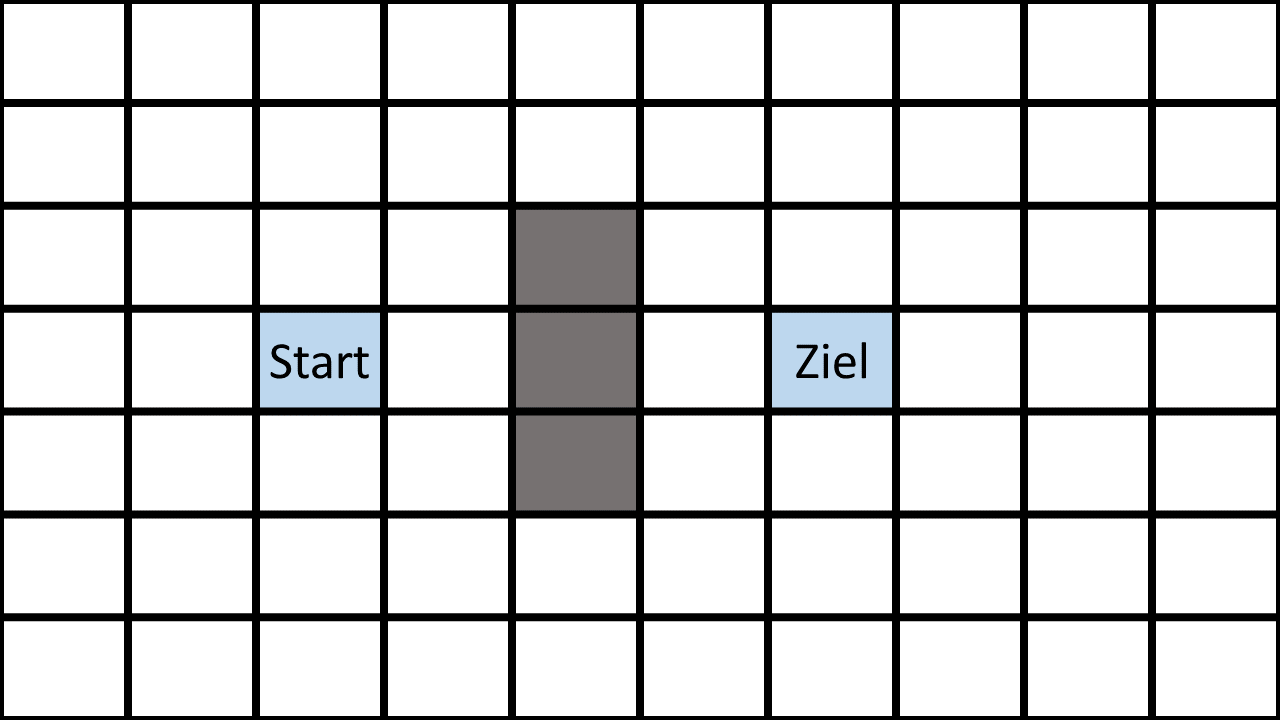
\includegraphics[width=\textwidth]{assets/aStarStep0.png}
        \caption{Schritt 1}
        \label{fig:aStartStep1}
    \end{subfigure}
    ~ %add desired spacing between images, e. g. ~, \quad, \qquad, \hfill etc. 
    %(or a blank line to force the subfigure onto a new line)
    \begin{subfigure}[b]{0.3\textwidth}
        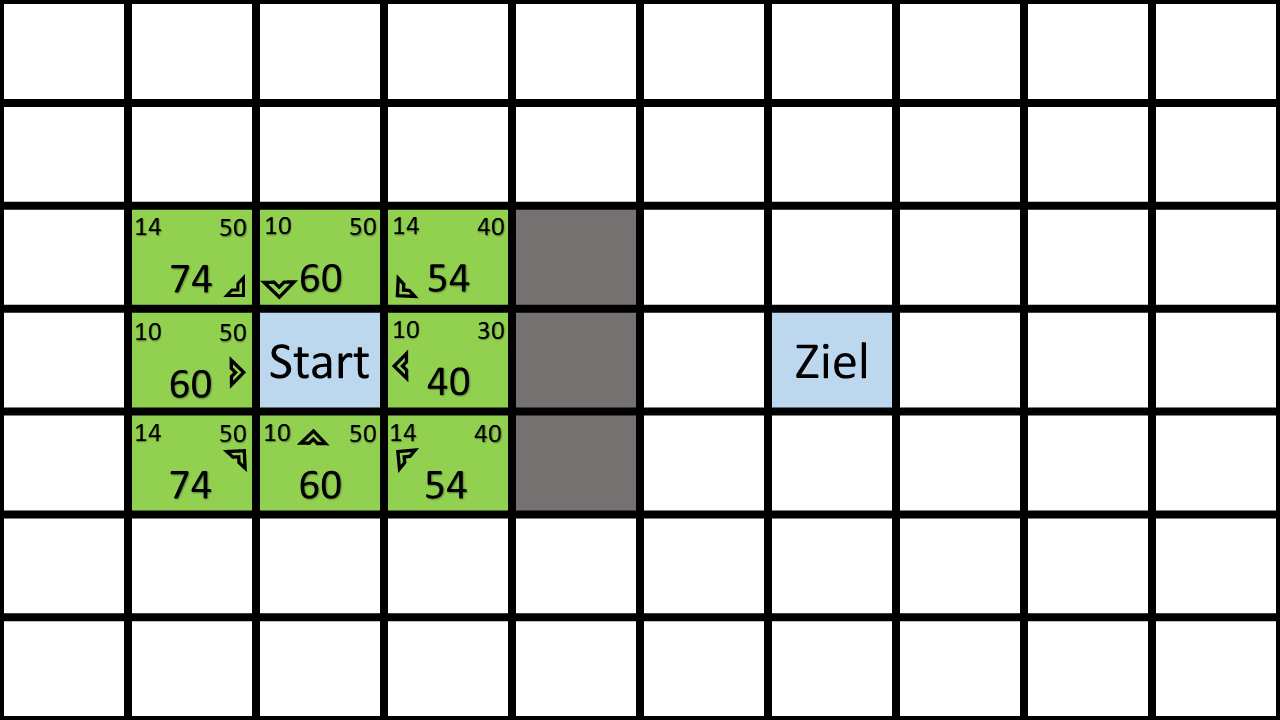
\includegraphics[width=\textwidth]{assets/aStarStep1.png}
        \caption{Schritt 2}
        \label{fig:aStartStep2}
    \end{subfigure}
    ~
    \begin{subfigure}[b]{0.3\textwidth}
        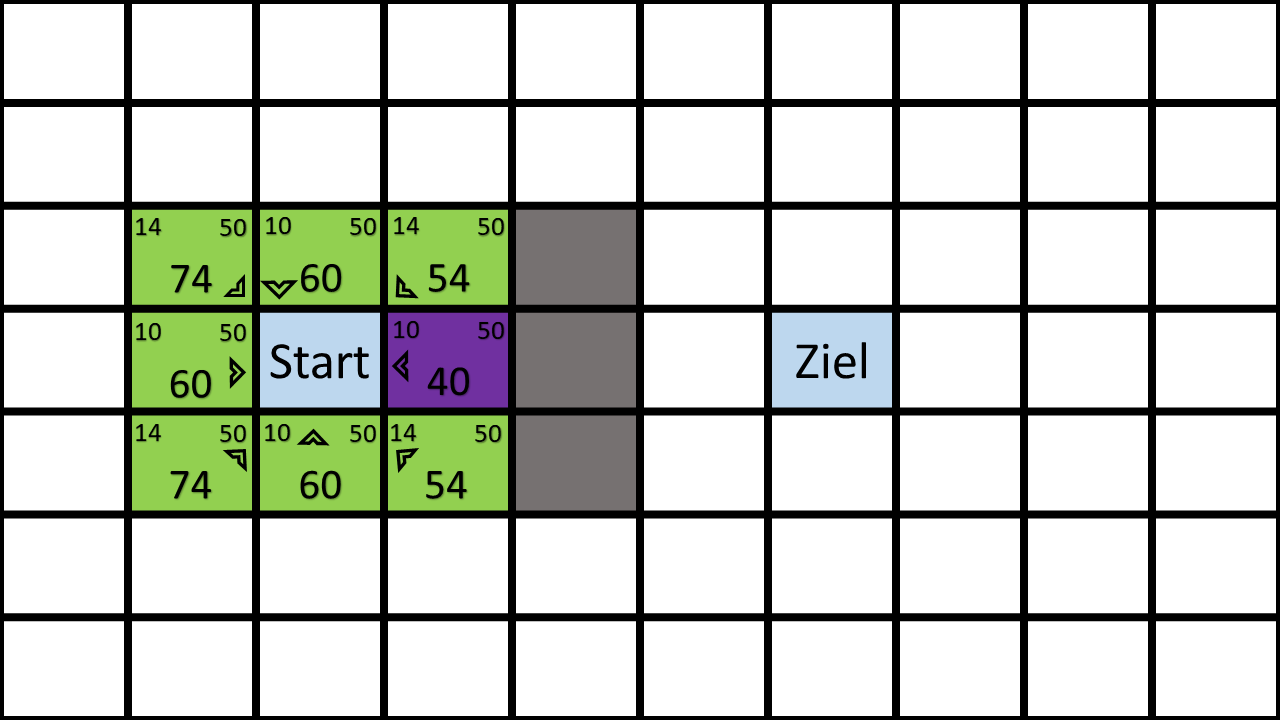
\includegraphics[width=\textwidth]{assets/aStarStep2.png}
        \caption{Schritt 3}
        \label{fig:aStartStep3}
    \end{subfigure}
    \caption{A* Ausführungsschritte 1-3}\label{fig:aStarStep1_3}
\end{figure}


\begin{figure}[H]
    \centering
    \begin{subfigure}[b]{0.3\textwidth}
        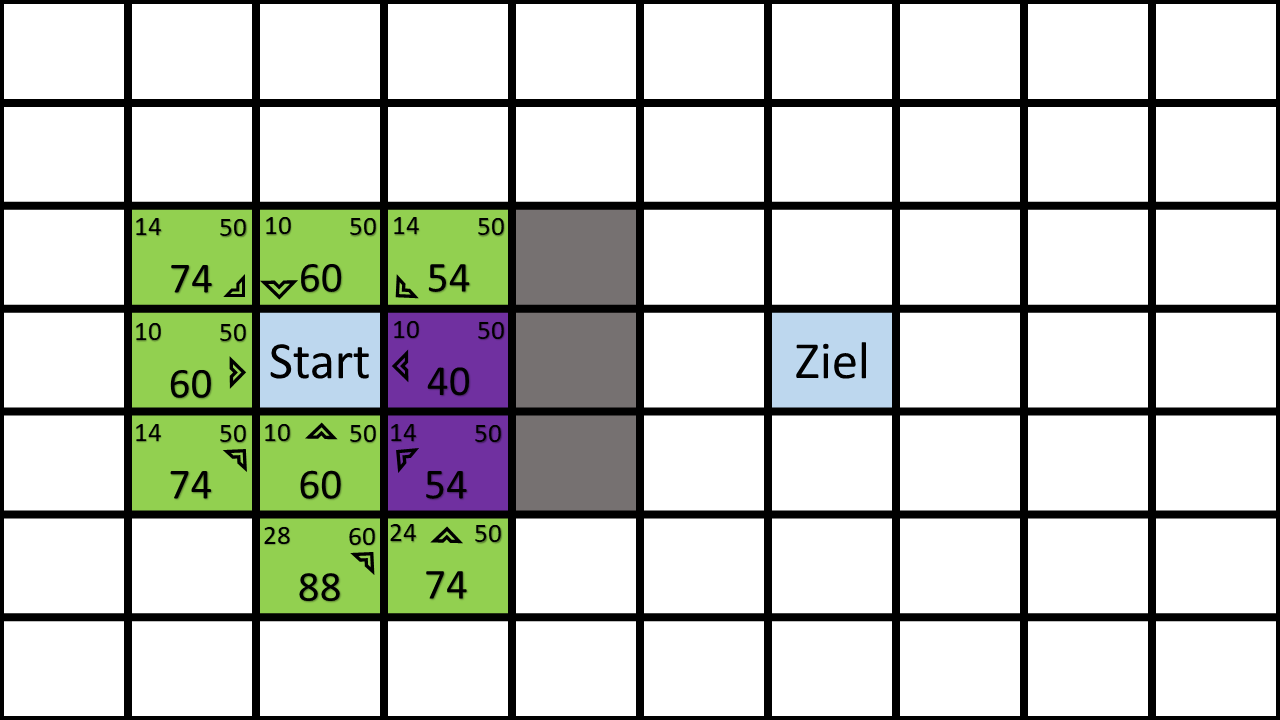
\includegraphics[width=\textwidth]{assets/aStarStep3.png}
        \caption{Schritt 4}
        \label{fig:aStartStep4}
    \end{subfigure}
    ~
    \begin{subfigure}[b]{0.3\textwidth}
        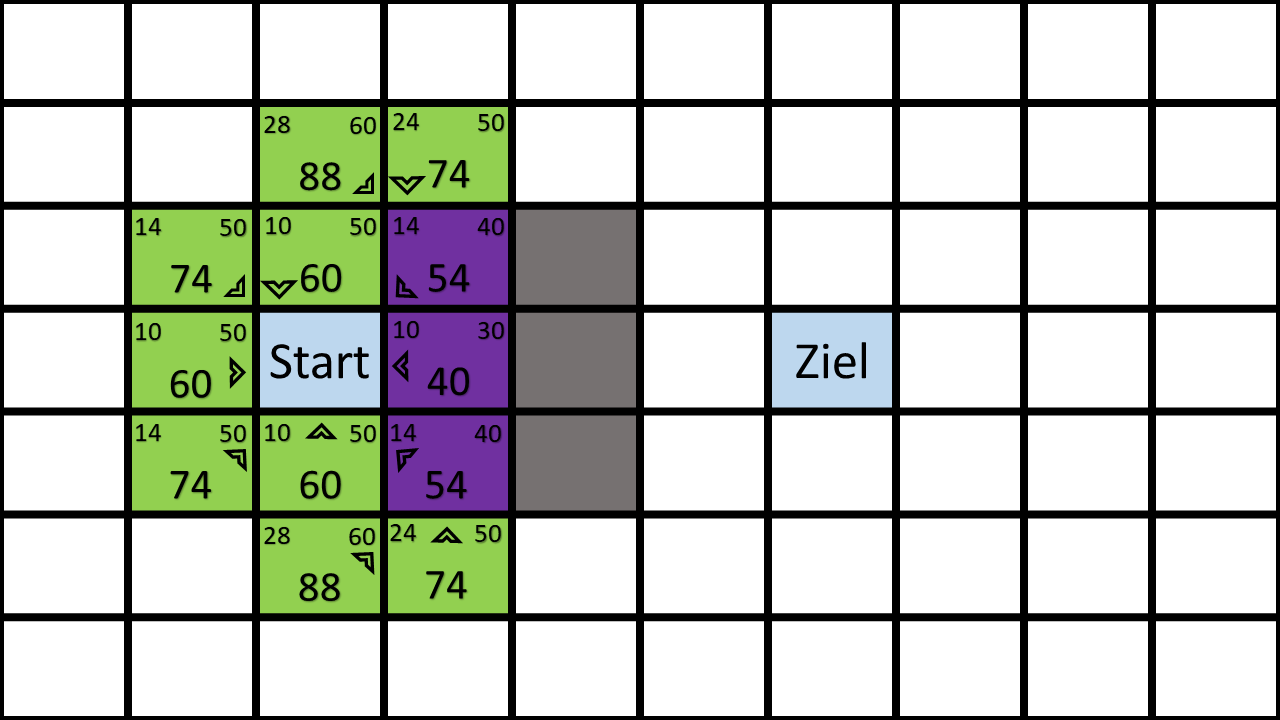
\includegraphics[width=\textwidth]{assets/aStarStep4.png}
        \caption{Schritt 5}
        \label{fig:aStartStep5}
    \end{subfigure}
    ~
    \begin{subfigure}[b]{0.3\textwidth}
        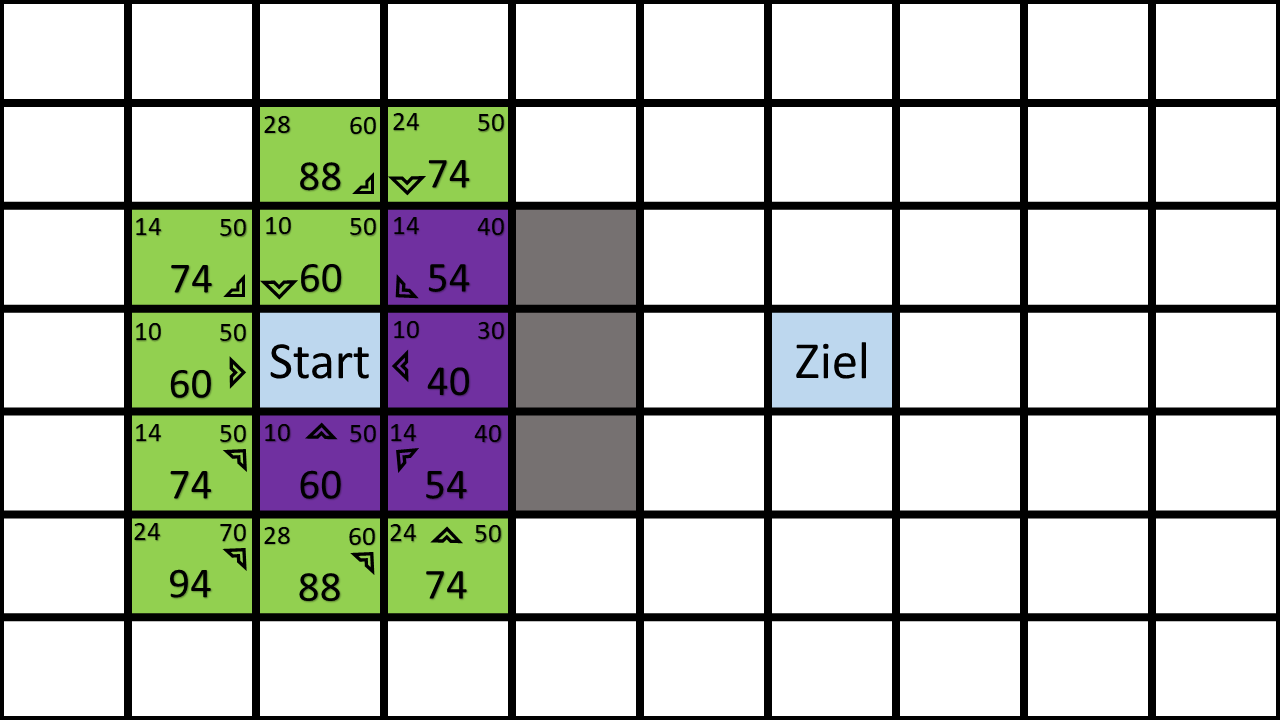
\includegraphics[width=\textwidth]{assets/aStarStep5.png}
        \caption{Schritt 6}
        \label{fig:aStartStep6}
    \end{subfigure}
    \caption{A* Ausführungsschritte 4-6}\label{fig:aStarStep4_6}
\end{figure}

\begin{figure}[H]
    \centering
    \begin{subfigure}[b]{0.3\textwidth}
        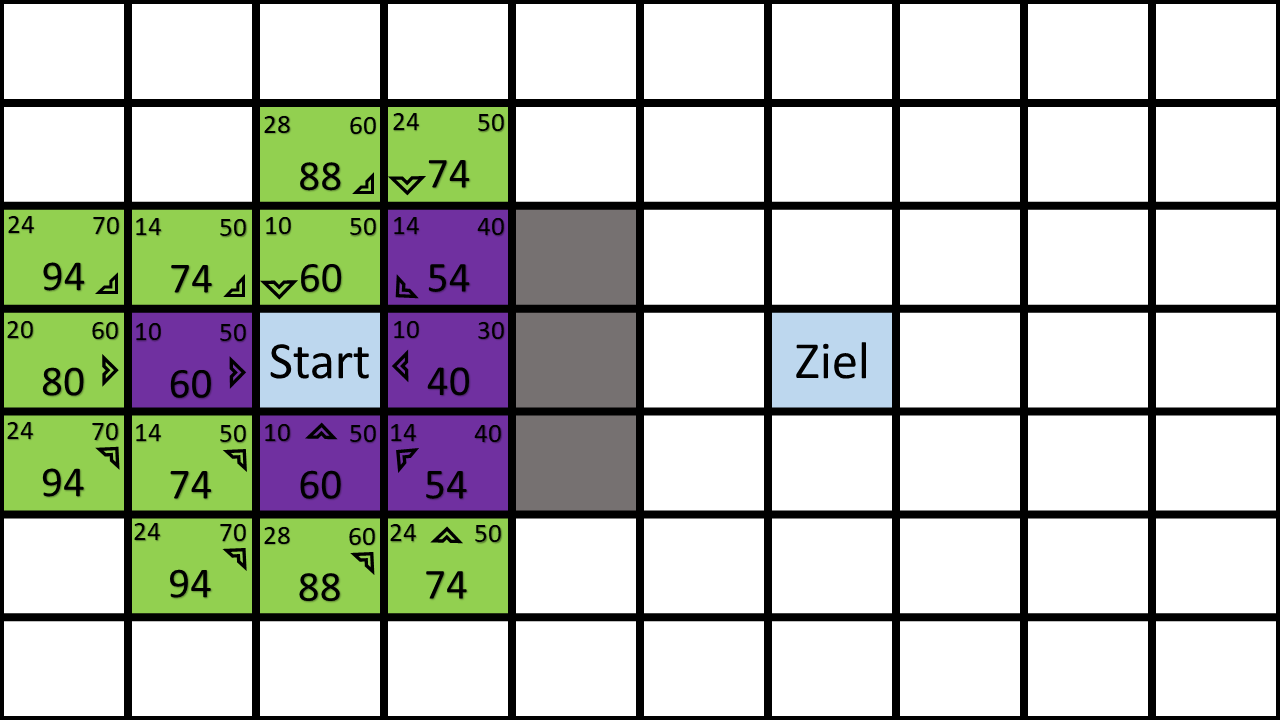
\includegraphics[width=\textwidth]{assets/aStarStep6.png}
        \caption{Schritt 7}
        \label{fig:aStartStep7}
    \end{subfigure}
    ~
    \begin{subfigure}[b]{0.3\textwidth}
        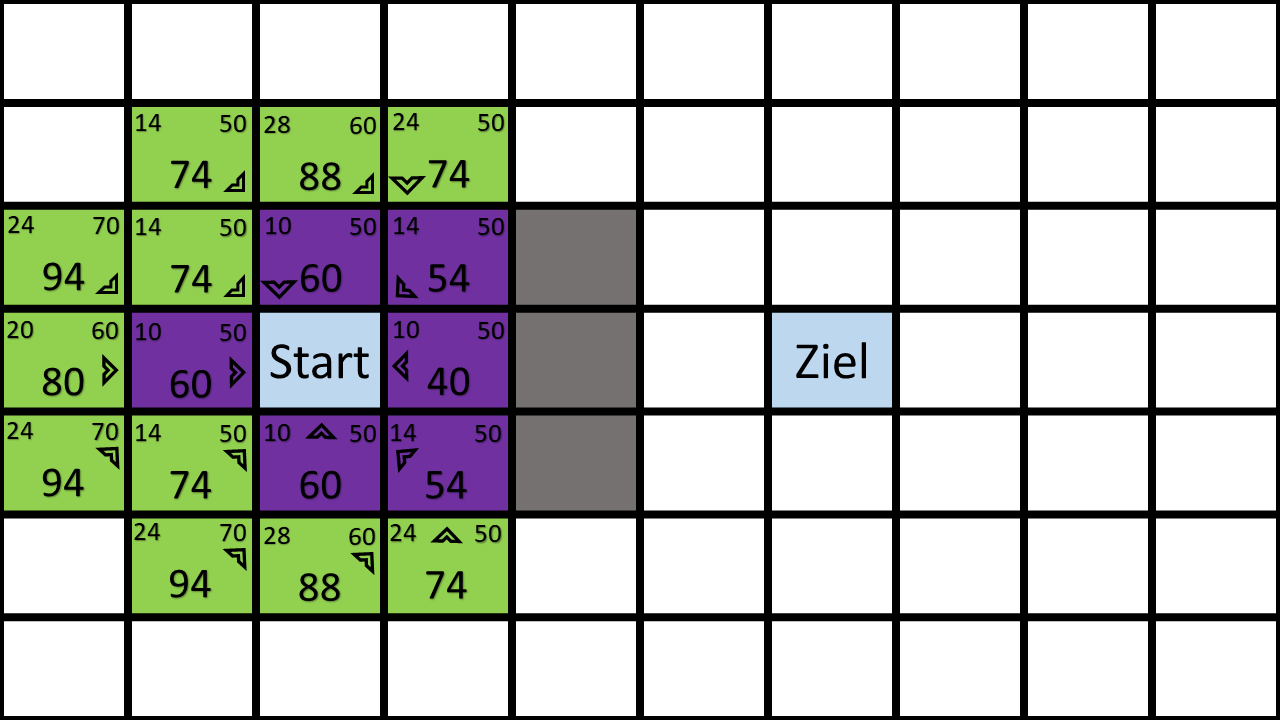
\includegraphics[width=\textwidth]{assets/aStarStep7.png}
        \caption{Schritt 8}
        \label{fig:aStartStep8}
    \end{subfigure}
    ~
    \begin{subfigure}[b]{0.3\textwidth}
        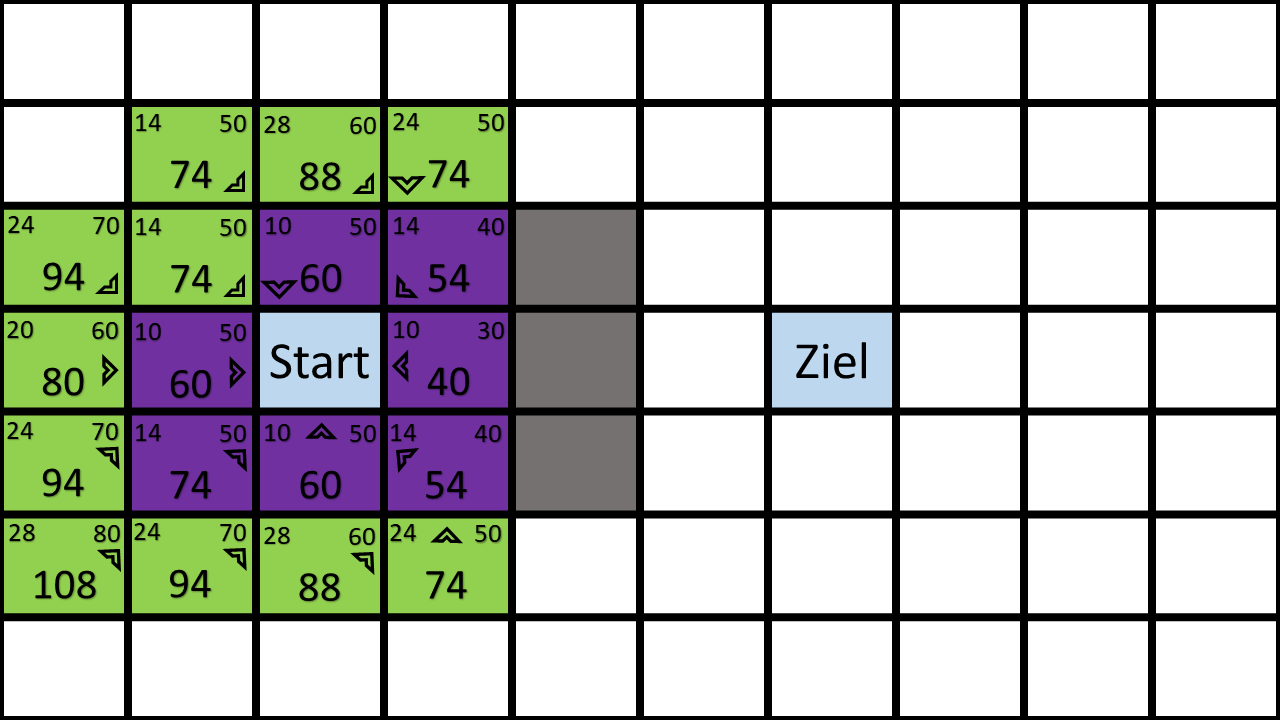
\includegraphics[width=\textwidth]{assets/aStarStep8.png}
        \caption{Schritt 9}
        \label{fig:aStartStep9}
    \end{subfigure}
    \caption{A* Ausführungsschritte 7-9}\label{fig:aStarStep7_9}
\end{figure}

\begin{figure}[H]
    \centering
    \begin{subfigure}[b]{0.3\textwidth}
        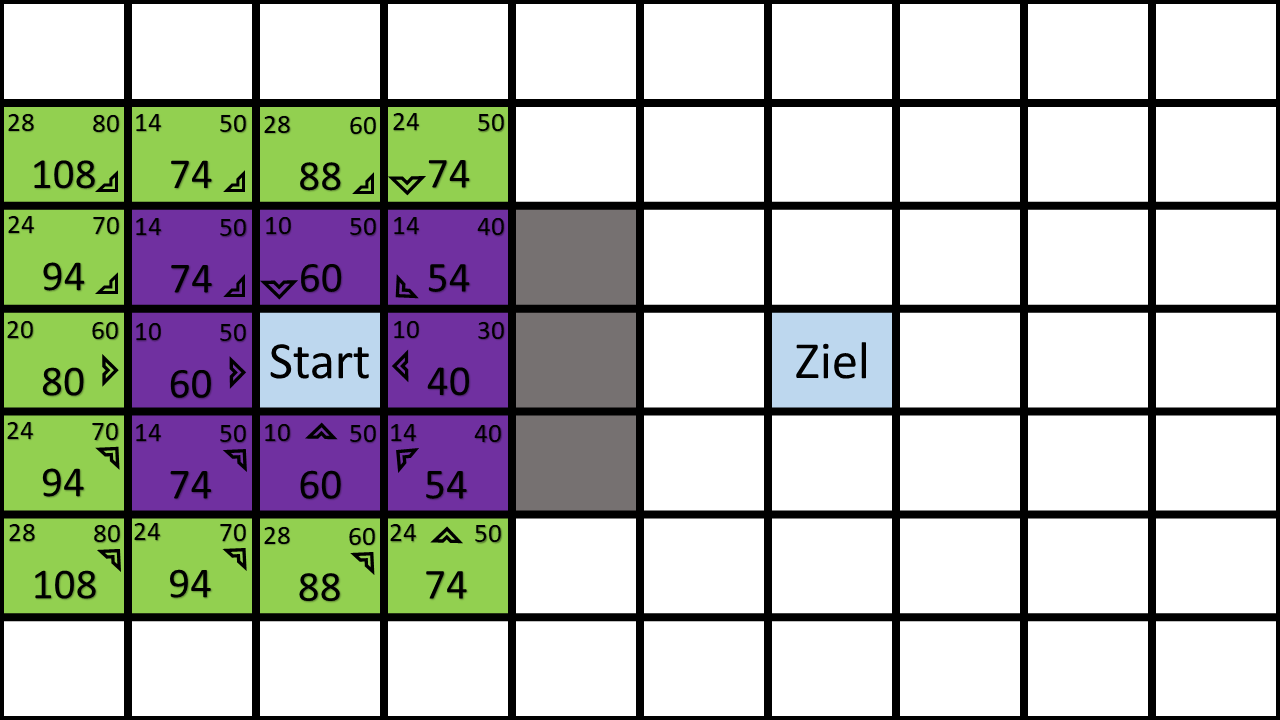
\includegraphics[width=\textwidth]{assets/aStarStep9.png}
        \caption{Schritt 10}
        \label{fig:aStartStep10}
    \end{subfigure}
    ~
    \begin{subfigure}[b]{0.3\textwidth}
        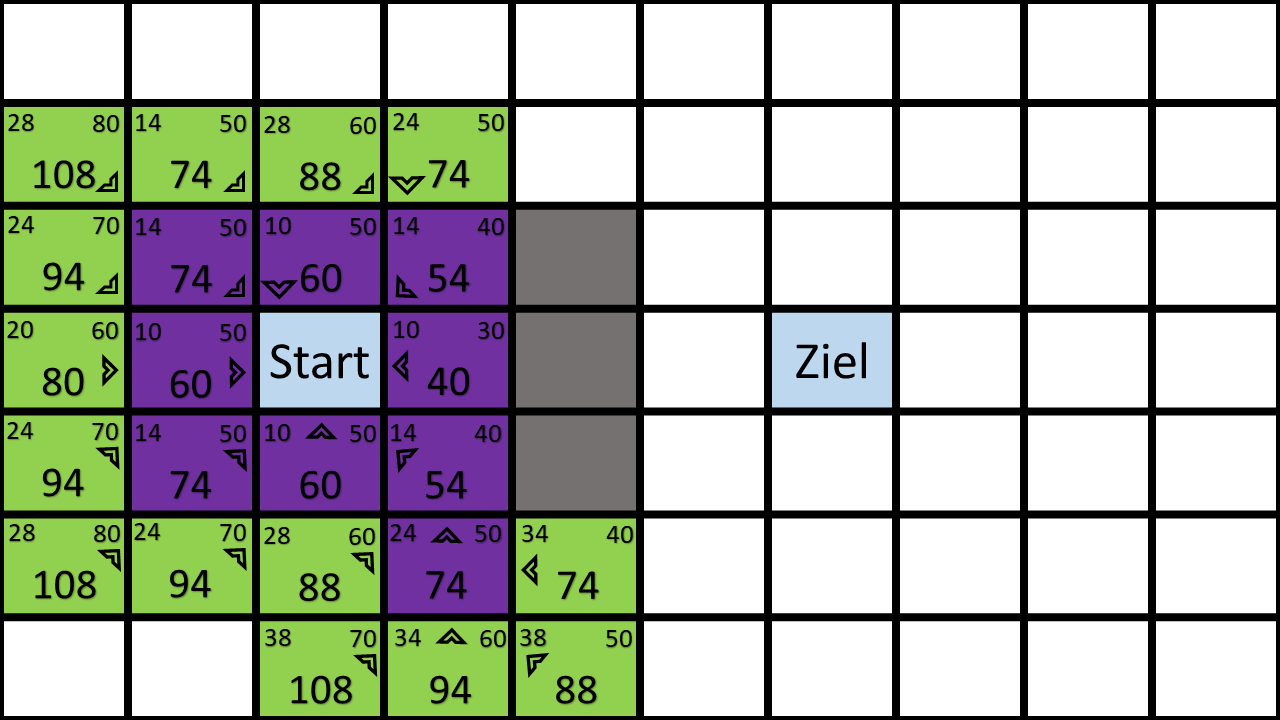
\includegraphics[width=\textwidth]{assets/aStarStep10.png}
        \caption{Schritt 11}
        \label{fig:aStartStep11}
    \end{subfigure}
    ~
    \begin{subfigure}[b]{0.3\textwidth}
        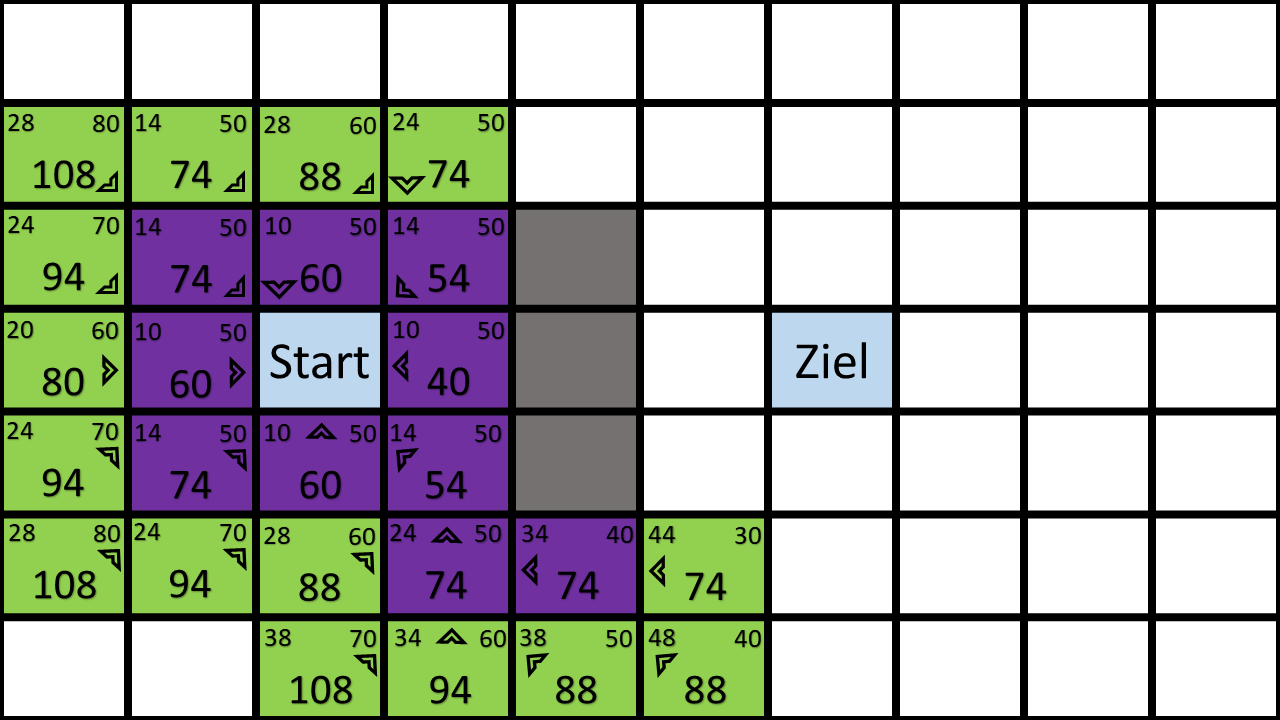
\includegraphics[width=\textwidth]{assets/aStarStep11.png}
        \caption{Schritt 12}
        \label{fig:aStartStep12}
    \end{subfigure}
    \caption{A* Ausführungsschritte 10-12}\label{fig:aStarStep10_12}
\end{figure}

\begin{figure}[H]
    \centering
    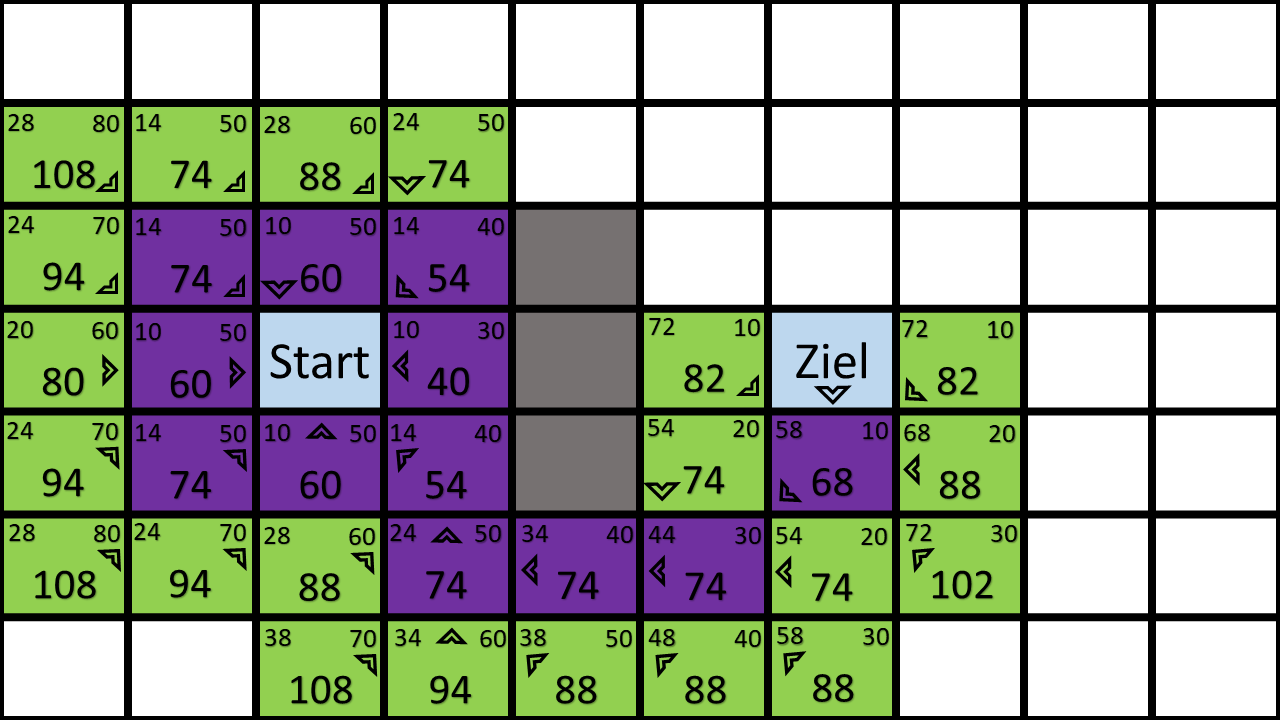
\includegraphics[width=\textwidth]{assets/aStarStep13.png}
    \caption{A* Schritt 13}\label{fig:aStarStep13}
\end{figure}

\label{sec:fundamentals}
\section{Unity}
\todo{Jannis - anlehnen an Vurals aus den Grundlagen)}
Unity ist eine GameEngine die in diesem Projekt genutzt wird, um das Spiel zu entwickeln. Des Weiteren besteht Unity aus einem sehr umfangreichen Editor, mit dem ein Spieleentwickler eine große Auswahl an Tools zur Entwicklung erh\"alt. Unity bietet sowohl die M\"oglichkeit in 2D, als auch in 3D zu entwickeln.

\section{Vuforia}
\subsection{ImageTargets}
\subsection{Object Recognition}
\subsubsection{Scanner}
\subsubsection{Erkennung}
